\documentclass{report}

% Language setting
% Replace `english' with e.g. `spanish' to change the document language
\usepackage[english]{babel}
\usepackage{blindtext}
\usepackage{titlesec}

% Set page size and margins
% Replace `letterpaper' with `a4paper' for UK/EU standard size
\usepackage[a4paper,top=2cm,bottom=2cm,left=3cm,right=3cm,marginparwidth=1.75cm]{geometry}

% Useful packages
\usepackage{float}
\usepackage{amsmath}
\usepackage{graphicx}
\usepackage{xcolor}
\usepackage[
colorlinks=true,urlcolor=blue,linkcolor=purple,citecolor=red
]{hyperref}

\usepackage[table,xcdraw]{xcolor}
\usepackage{adjustbox}

\usepackage{csquotes}
\usepackage[
backend=biber,
style=ieee,
]{biblatex}
\addbibresource{sample.bib}

\usepackage[Conny]{fncychap}
%\ChNameAsIs
\ChTitleAsIs
\pagestyle{headings}

\title{Scalable IoT Systems based on OpenRemote \\Project plan}
\author{Vladislav Serafimov}

\begin{document}
	\maketitle
	
	
	
	\tableofcontents
	
	\chapter{Introduction}
	This chapter introduces the foundational concepts behind the assignment.
	\section{Background}
	The assignment was created by the Ambient Intelligence (AmI) research group in order to expand on the current knowledge in the Internet of Things (IoT) research area. AmI has worked on a number of IoT projects related to sports, safety and industry. Their aim is to make environments more interconnected, by monitoring them, processing the data and feeding it to the user.
	
	The student thesis project is a part of NOWATT, which is a collaboration between academia and industry. The NOWATT project involves both AmI and the company behind the OpenRemote \footnote{OpenRemote is an open-source device management platform; for more information see \href{https://openremote.io}{this link}} platform. Because the multi-organization team would like to use OpenRemote and integrate it into their future work.
	
	\section{Purpose of the assignment}\label{purpose}
	The assignment is designed with the intention of expanding on what AmI has already been researching. Its main purpose is to develop scalable IoT systems using OpenRemote and to do so with clear visualization.
	
	There are three main parts that make up the assignment. The first one is deploying an OpenRemote instance and simulating IoT devices that communicate with it. An MQTT \footnote{MQTT stands for Message Queuing Telemetry Transport \cite{mqtt_wiki}. It is a communication protocol, mainly used for purposes relating to IoT.} setup needs to be realized, over which the data needs to be transferred from the mock devices to OpenRemote. The second part of the assignment is edge computing optimizations. They are another crucial part of the assignment, as the processing that is not done on the cloud needs to be as fast and resource-efficient as possible. Lastly, in order to test and verify the proper working of the devices, the sensor data needs to be extracted and validated by generating graphical representations of it. The data gathered throughout the project will also need to be analyzed using statistical models. These two tasks will be a part of the testing activity (see Chapter\ref{end_phase}).
	
	If there is time left after finalizing the core of the project, data prediction using machine learning can also be implemented. Firmware for IoT devices is another feature that can also be developed, if there is enough time.
	
	\section{Assignment specifications}\label{specifications}
	Figure \ref{openremote_diagram} shows a diagram of all the functionalities offered by OpenRemote. In brief, OpenRemote is a platform for managing IoT devices. The most important features for this project are the MQTT agents (functioning as brokers/clients) and the built-in data visualization options. 
	
	\begin{figure}[ht]
		\centering
		%\includegraphics[width=1\linewidth]{openremote_diagram.jpg}
		\caption{OpenRemote application diagram \cite{openremote_intro}}
		\label{openremote_diagram}
	\end{figure}
	
	The languages used for this project will be Python and C/C++. The extensive and varied catalog of Python packages makes the language better for tasks where simplicity is valued over speed. Because of this, during the project, Pyhton will be used for modeling and visualization of the data. The MQTT communication can be done using both, which means they need to be evaluated during the project to see which one suits it better.
	
	Data visualization and modeling will both be done, at least partially, in Python. `matplotlib` is one of the most widely-used packages for data visualization and because of this it was chosen for this project as well. Because OpenRemote has built in features for data plotting, it will also be used for some visuals. Data modeling, using statistical models, will be done in order to make sure the final product is configured in the optimal way. The optimal configuration will balance performance and service availability. Python's relevant features are the reason it was chosen for this task as well. 
	
	The extra features will use the same languages. C/C++ is more suited to low-level applications, so it will be used for the firmware. Python has a plethora of features and packages that make it good specifically for machine learning, so data prediction will be done in Python.
	
	
	\section{Methodological approach}\label{methodological_approach}
	The waterfall model (see Figure \ref{phases}) was selected for this project. It is a straightforward model that is suited for assignments where the requirements do not undergo any significant changes. This is the case in this project, because the output needs to align with the goals of the overarching project AmI is working on. Another relevant strength of this model is that adhering to the methodology does not require much effort to implement once the groundwork is laid. Other models, like Scrum, require a lot of time and energy to be implemented properly, but in the waterfall model every stage follows up on what the previous set up. What is more, the chosen model is excellent for documentation. The straightforward approach to the project means there will be no retroactive editing of existing documentation. This leads to a situation where the documentation product of each phase will lead into the next. 
	
	\begin{figure}[h]
		\centering
		%\includegraphics[width=\linewidth]{phases.png}
		\caption{Project phases using the waterfall model}
		\label{phases}
	\end{figure}
	
	
	\chapter{Products and project objectives}
	This chapter describes all the required products and based on them sets up the objectives for the project.
	
	\section{Products}
	There are two types of products that need to be delivered: professional products and learning products.
	
	The professional products consist of several deliverables, which need to be provided to AmI after completion of the project. The main deliverable of the project is the firmware code. Just as important are the data extraction and visualization scripts. The edge computing optimizations should also be documented and reported as a part of the final product. The final report is also an important product, as future work will require some foundation to base further research on.
	
	The learning products are there to ensure the student (see Table \ref{involved}) has completed the learning goals for the project. The final report is also an important part of the learning products, as it demonstrates knowledge and the ability to communicate that knowledge. Another important deliverable is the learning report, which is an introspection about the project and its highlights. The last deliverable is the final presentation PowerPoint file, which is not as important as the oral presentation. However, it is still a demonstration of the acquired knowledge and skills during the project.
	
	\section{Objectives}
	As the chief goal of the project is to expand AmI's pool of knowledge, the project objectives need to align with that goal. It is also important to note that the project is done as a graduation assignment, which means there are learning objectives to be completed in parallel with the professional objectives. 
	
	The SMART\footnote{SMART in this case stands for Specific, Measurable, Achievable, Relevant, Time-bound} method for setting goals cab be applied to this project. The goals can be made even more specific by using the mandatory deliverables for the project. SMART will simplify the bookkeeping of the whole project.
	
	\begin{itemize}
		\item Goal \#1: Complete the learning objectives of the project.
		\item Goal \#2: Complete the professional objectives of the project.
	\end{itemize}
	
	\subsection{Learning objectives}
	\begin{enumerate}
		\item Project plan: outline of the project
		\item Technical report: technical documentation of the project
		\item Learning report: reflection on the project as a learning activity
		\item Final presentation (incl. presenting): communication of the highlights of the project 
	\end{enumerate}
	
	\textbf{SMART}
	\begin{itemize}
		\item Specific: The deliverables associated with the learning objectives all have to be completed by the student and submitted for review to Saxion. The only exception is the final presentation, which includes both the digital presentation and the in-person presenting done by the student. The learning objectives are set in place so that the student can demonstrate sufficient knowledge and skills in order to obtain a diploma.
		\item Measurable: Every deliverable has a corresponding grading rubric, which quantifies the proficiency of the student.
		\item Achievable: The learning objectives build on top of the knowledge that the student has acquired during their study at Saxion. In order to navigate any setbacks that concern the learning objectives, the student can request feedback from the Saxion coach. All other work can be completed by the student with the use of the internet and all publicly available tools and resources.   
		\item Relevant: Goal \#1 is aligned with the degree of the student. Learning objectives are set in place to showcase to what level the student has mastered the knowledge and competences acquired during the study.
		\item Time-bound: Every submission has its own due date, consult Chapter \ref{plan} for more information.
	\end{itemize}
	\subsection{Professional objectives}
	\begin{enumerate}
		\item Code: main deliverable; includes everything from firmware to scripts
		\item Visualizations: graphs corroborating the findings of the project
		\item Documentation: a document covering the findings of the project and how to work with the code  
	\end{enumerate}
	
	\textbf{SMART}
	\begin{itemize}
		\item Specific: The professional objectives were discussed with the company coach before the technical work on the project was started. The main goal of the project is to test the scalability of OpenRemote in order to prove whether or not it can be used in future (industrial) IoT projects carried out by AmI. The auxiliary goals, set in place to ensure the findings of the project are as truthful and useful as possible, are discussed in Chapters \ref{specifications} and \ref{project_boundaries}
		\item Measurable: The project should result in clear visualizations and numbers. These outcomes should show how the speed and stability of OpenRemote scale with the number of devices. The analysis that can be performed on this data should result in an answer to the question "Is OpenRemote scalable enough?".  
		\item Achievable: The student has the skillset to conduct the technical part of the project successfully. The physical tools that the project requires will all be provided by AmI. AmI also provides technical support in the form of the company coach.
		\item Relevant: The project is a part of a bigger project within AmI called NOWATT. The results of the professional objectives will directly utilized by the NOWATT team. 
		\item Time-bound: The timeline for the professional objectives needs to align with that for the learning objectives. This is so, because the project is done as a graduation assignment and the graduation deadlines are mandated by Saxion.
	\end{itemize}
	
	
	
	
	\chapter{Project activities}
	For the sake of simplicity the project can be broken down into 3 phases as seen in Figure \ref{phases}. Those phases are the start phase, realization phase and finalization/end phase. This simplification helps with the scheduling of the tasks. There is a task, which needs to be done throughout all phases and that task is documentation. Due to the use of the waterfall model (see Chapter \ref{methodological_approach}), every phase of the documentation activity seamlessly flows into the next. Because of this, it is indicated as separate in Figure \ref{phases}.
	
	
	\section{Start phase}
	The start phase includes the first 2 blocks of the waterfall model (see Figure \ref{methodological_approach}). The familiarization involves getting acquainted with AmI's technical requirements and what technology they expect to be involved in the project. What is even more crucial in this period is getting familiar with the assignment and making sure the plan meets AmI's expectations. After concluding the process of familiarization, the research phase can start. It involves exploration of material that can help with building the solution and possibly looking into similar problems and their solutions. 
	
	There are also several documentation activities during this phase. These activities include scheduling, risk analysis and the project plan. 
	\section{Realization phase}
	This phase is the longest and most important of the three. The assignment should be mostly completed during this phase. The first part of realization involves implementing the different parts of the final product (firmware, visualizations of mock data, etc.). The second part is about combining the separate implementations into a single, mostly-finished, product.
	
	Alongside the formerly mentioned tasks, the technical report needs to be worked on as well. The learning report should also be started before the end of the realization phase. The technical report will be prioritized over the learning report, as it requires more time and effort. The code will also require some documentation, in order to aid future work that extends the functionality of the products of this project. 
	
	\section{End phase}\label{end_phase}
	While some amount of testing will be done during realization, holistic tests can only be performed once the integration activity has concluded. After testing and fixing the product, the finalization activity can begin. During this activity, all the minor details that need attention will be addressed (e.g. code formatting).
	
	During the end phase, and especially during the finalization, a lot of documentation will need to be done. Two separate presentations, one for AmI and one for Saxion, will need to be made and presented. The technical and learning report, as well as all the code documentation, will need to be finalized. 
	
	\chapter{Project boundaries} \label{project_boundaries}
	The project boundaries were initially brainstormed based on the contents of Chapters \ref{purpose} and \ref{specifications}. After that, they were discussed with the client to ensure both parties were aware of the other's expectations. 
	
	\textbf{Must have}
	\begin{itemize}
		\item Sensor data extraction
		\item OpenRemote integration
	\end{itemize}
	
	\textbf{Should have}
	\begin{itemize}
		\item Visualizations using sensor data
		\item MQTT configuration
	\end{itemize}
	
	\textbf{Could have}
	\begin{itemize}
		\item Physical device implementation
		\item Data prediction using machine learning
		\item Firmware implementation for emulated devices
	\end{itemize}
	
	\textbf{Will not have}
	\begin{itemize}
		\item Cross-platform compatibility
		\item Several implementations for different hardware platforms 
		\item Cloud-based processing
	\end{itemize}
	
	
	\chapter{Quality assurance}\label{quality_assurance}
	The quality of the project and the resulting products is of the utmost importance. 
	
	To guarantee the quality of the technical product, a lot of testing needs to be done. As discussed in Chapter \ref{end_phase}, tests will be conducted during implementation and integration, but the main testing activity will be conducted during the end phase of the project. This method of working was chosen in order to maximize the chance of spotting issues with the products.
	
	In order for the student to remains productive, several safeguards need to be put in place. Frequent communication between the student and the company coach (as discussed in Chapter \ref{communication}) is one of the most vital safeguards. It guarantees both parties are well-informed and might help resolve issues if any arise during the project. Another important factor for the student's performance is the work environment. Because of the preferences of both the student and the client, most of the work hours will be done on location in one of AmI's rooms. Most of the project work can also be done remotely, if the need arises.
	
	
	
	\chapter{Project organization}
	The project organization chapter discusses the different parties involved in this project and how they are expected to interact.
	
	\section{Organization}
	
	\begin{table}[h]
		\centering
		\begin{tabular}{|l|l|l|}
			\hline
			Name                & Work email              & Role          \\ \hline
			Vladislav Serafimov & v.serafimov@saxion.nl   & Student       \\ \hline
			Yanin Kasemsinsup   & y.kasemsinsup@saxion.nl & Saxion coach  \\ \hline
			Eyuel Ayele         & e.d.ayele@saxion.nl     & Company coach \\ \hline
		\end{tabular}
		\caption{People involved in the project}
		\label{involved}
	\end{table}
	
	The student is the person doing the assignment. They are responsible for the deliverables. Furthermore, they should be the initiator and proactively seek out the Saxion and company coach, if necessary. The Saxion coach is in charge of grading and is responsible for supporting the learning needs of the student. The company coach has similar tasks, with a few key differences. Both coaches participate in the grading, but their responsibilities vary depending on the deliverable. The exact differences are not relevant and will not be discussed in this report. The most important difference between the two coaches is that while the Saxion coach provides learning support, the company coach is responsible for the technical support of the student. The company coach also serves as a supervisor and as such makes sure the student is working on the project in a manner similar to the agreements made in the contract and the project plan. There will also be meetings with the Saxion coach to ensure the learning goals are met and that the products required by Saxion will be delivered in a timely manner.
	
	\section{Communication} \label{communication}
	The communication will mainly be done online. This enables easier sharing of files and data. However, physical meetings between the student and the company coach are crucial for the success of the project. In order to ensure the quality and consistency of the student's work, these meetings will be held often in the beginning of the project. As time goes on, less of these meetings will be needed to maintain the same level of quality.
	
	\chapter{Planning}\label{plan}
	This chapter discusses the scheduling of the project. The schedule was created using a Gantt chart (see Figure \ref{fig:gantt}), which contributes to the established structure of the project.
	
	The deliverables are also a part of the planning. The project plan should be done a week before the end of the start phase. Using in, the functional and technical design chapters of the technical report can be completed. The report can then be submitted before the start of the finalization activity, aong with the code, visualizations and all other technical deliverables. The final presentation needs to be delivered within the first week of the the finalization activity. To ensure delays do not cause problems with meeting deadlines, all the dates have a buffer time of about a week.
	
	\begin{figure}[h]
		\centering
		%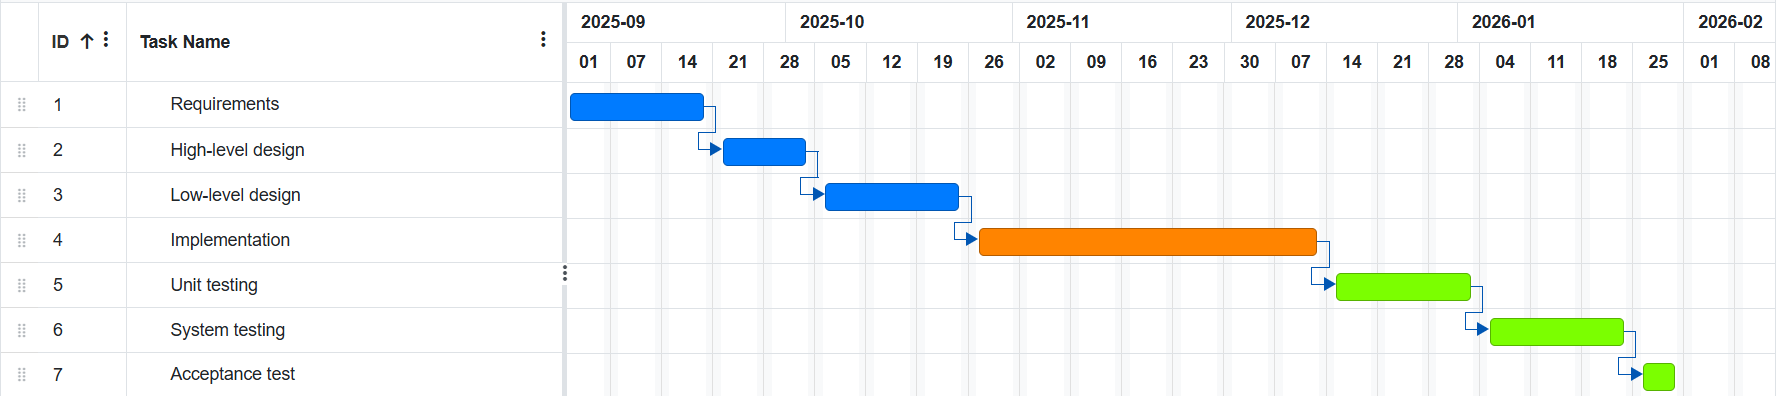
\includegraphics[width=1\linewidth]{gantt.png}
		\caption{Gantt chart}
		\label{fig:gantt}
	\end{figure}
	
	
	%\chapter{Costs and benefits}
	
	\chapter{Risk analysis}
	This chapter discuses the most common risks that might occur during a project like this and ways to address them. For a more detailed risk analysis, see \href{run: ./risk_analysis.xlsm}{the attached MS Excel file}. 
	
	
	\begin{table}[h]
		\centering
		\begin{adjustbox}{angle=-90}
			\begin{tabular}{|l|l|l|l|l|l|}
				\hline
				Risk                                                              & Description                                                                                                                                          & \begin{tabular}[c]{@{}l@{}}Frequency/\\ Probability\end{tabular} & Severity                       & Importance                     & Risk mitigation                                                                                                                                        \\ \hline
				Software issues                                                   & \begin{tabular}[c]{@{}l@{}}Bugs might get \\ through testing\end{tabular}                                                                            & \cellcolor[HTML]{34FF34}Low                                      & \cellcolor[HTML]{F8FF00}Medium & \cellcolor[HTML]{FE0000}High   & See Chapter \ref{quality_assurance}                                                                                                                    \\ \hline
				Hardware issues                                                   & \begin{tabular}[c]{@{}l@{}}Hardware might \\ malfunction\end{tabular}                                                                                & \cellcolor[HTML]{34FF34}Low                                      & \cellcolor[HTML]{FE0000}High   & \cellcolor[HTML]{F8FF00}Medium & \begin{tabular}[c]{@{}l@{}}Results of the tests with \\ the physical devices need\\ to be compared with the \\ simulations\end{tabular}                \\ \hline
				Time management                                                   & \begin{tabular}[c]{@{}l@{}}Unexpected \\ events might\\ cause delays\end{tabular}                                                                    & \cellcolor[HTML]{34FF34}Low                                      & \cellcolor[HTML]{34FF34}Low    & \cellcolor[HTML]{F8FF00}Medium & \begin{tabular}[c]{@{}l@{}}Every event in the \\ schedule has a buffer \\ in order to mitigate\\ the impact of delays\end{tabular}                     \\ \hline
				\begin{tabular}[c]{@{}l@{}}Hardware \\ availability\end{tabular}  & \begin{tabular}[c]{@{}l@{}}Required hardware \\ components might \\ not be available\end{tabular}                                                    & \cellcolor[HTML]{34FF34}Low                                      & \cellcolor[HTML]{FE0000}High   & \cellcolor[HTML]{34FF34}Low    & \begin{tabular}[c]{@{}l@{}}Using alternative suppliers \\ and/or components makes \\ the likelihood of this being \\ a serious hurdle low\end{tabular} \\ \hline
				\begin{tabular}[c]{@{}l@{}}Deployment \\ issues\end{tabular}      & \begin{tabular}[c]{@{}l@{}}The OpenRemote \\ instance and the \\ Python code might \\ interact in an \\ unexpected way \\ on the server\end{tabular} & \cellcolor[HTML]{34FF34}Low                                      & \cellcolor[HTML]{F8FF00}Medium & \cellcolor[HTML]{34FF34}Low    & \begin{tabular}[c]{@{}l@{}}Docker needs to be used along\\ with good networking practices\end{tabular}                                                 \\ \hline
				\begin{tabular}[c]{@{}l@{}}Unrealistic\\ simulations\end{tabular} & \begin{tabular}[c]{@{}l@{}}The real hardware \\ might behave \\ differently from \\ the simulations\end{tabular}                                     & \cellcolor[HTML]{F8FF00}Medium                                   & \cellcolor[HTML]{34FF34}       & \cellcolor[HTML]{F8FF00}Medium & \begin{tabular}[c]{@{}l@{}}Different simulations with different\\ levels of abstraction can solve this\\ issue\end{tabular}                            \\ \hline
			\end{tabular}
		\end{adjustbox}
		\caption{Risk analysis table}
		\label{risk_analysis}
	\end{table}
	
	The most critical issues that need to be prevented are those relating to hardware. This is because they have the biggest impact on the project, as seen in Table \ref{risk_analysis}. In order to lessen the impact of a hardware issues and supply shortages, it was decided that the software should work on a simulation before being tested on a real piece of hardware. Simulating on different levels of abstraction can help simplify the implementation of the MQTT connection and later when a working connection has been established, a more realistic and intricate hardware simulation can be done. This way, if there is a supply shortage and there are no alternative distributors, the code can still be verified more accurately. In case of hardware issues, having simulations and an expected result will mean these issues can be diagnosed early on. This has the potential of saving a lot of time later in the project.   
	
	
	\printbibliography
	
\end{document}